\section{XMFrame  Class Reference}
\label{classXMFrame}\index{XMFrame@{XMFrame}}
{\tt \#include $<$XMManagers.h$>$}

Inheritance diagram for XMFrame::\begin{figure}[H]
\begin{center}
\leavevmode
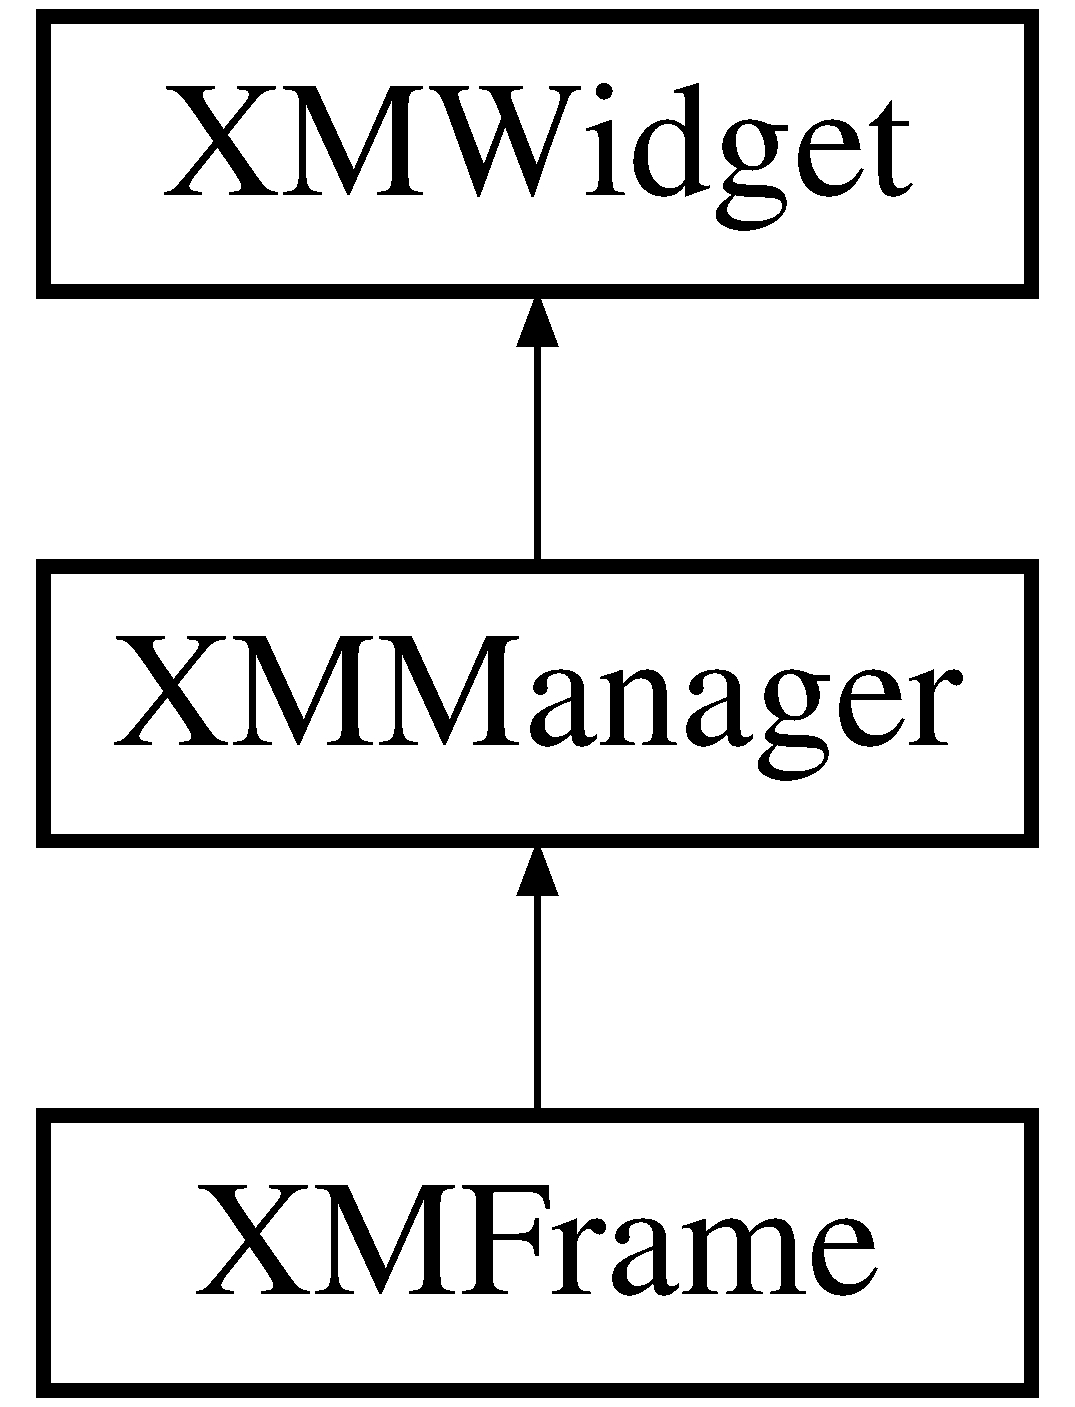
\includegraphics[height=3cm]{classXMFrame}
\end{center}
\end{figure}
\subsection*{Public Methods}
\begin{CompactItemize}
\item 
{\bf XMFrame} (char $\ast${\bf name})
\item 
{\bf XMFrame} (Widget {\bf id})
\item 
{\bf XMFrame} (char $\ast$n, {\bf XMApplication} \&parent, Arg\-List l=NULL, Cardinal num\_\-args=0)
\item 
{\bf XMFrame} (char $\ast$n, {\bf XMWidget} \&parent, Arg\-List l=NULL, Cardinal num\_\-args=0)
\item 
{\bf XMFrame} (char $\ast$n, Widget parent, Arg\-List l=NULL, Cardinal num\_\-args=0)
\item 
void {\bf Margins} (Dimension height, Dimension width=0)
\item 
void {\bf Set\-Shadow\-Type} (unsigned char type)
\end{CompactItemize}


\subsection{Constructor \& Destructor Documentation}
\index{XMFrame@{XMFrame}!XMFrame@{XMFrame}}
\index{XMFrame@{XMFrame}!XMFrame@{XMFrame}}
\subsubsection{\setlength{\rightskip}{0pt plus 5cm}XMFrame::XMFrame (char $\ast$ {\em name})\hspace{0.3cm}{\tt  [inline]}}\label{classXMFrame_a0}




Definition at line 425 of file XMManagers.h.

References XMWidget::name.\index{XMFrame@{XMFrame}!XMFrame@{XMFrame}}
\index{XMFrame@{XMFrame}!XMFrame@{XMFrame}}
\subsubsection{\setlength{\rightskip}{0pt plus 5cm}XMFrame::XMFrame (Widget {\em id})\hspace{0.3cm}{\tt  [inline]}}\label{classXMFrame_a1}




Definition at line 426 of file XMManagers.h.

References XMWidget::id.\index{XMFrame@{XMFrame}!XMFrame@{XMFrame}}
\index{XMFrame@{XMFrame}!XMFrame@{XMFrame}}
\subsubsection{\setlength{\rightskip}{0pt plus 5cm}XMFrame::XMFrame (char $\ast$ {\em n}, {\bf XMApplication} \& {\em parent}, Arg\-List {\em l} = NULL, Cardinal {\em num\_\-args} = 0)\hspace{0.3cm}{\tt  [inline]}}\label{classXMFrame_a2}




Definition at line 427 of file XMManagers.h.\index{XMFrame@{XMFrame}!XMFrame@{XMFrame}}
\index{XMFrame@{XMFrame}!XMFrame@{XMFrame}}
\subsubsection{\setlength{\rightskip}{0pt plus 5cm}XMFrame::XMFrame (char $\ast$ {\em n}, {\bf XMWidget} \& {\em parent}, Arg\-List {\em l} = NULL, Cardinal {\em num\_\-args} = 0)\hspace{0.3cm}{\tt  [inline]}}\label{classXMFrame_a3}




Definition at line 430 of file XMManagers.h.\index{XMFrame@{XMFrame}!XMFrame@{XMFrame}}
\index{XMFrame@{XMFrame}!XMFrame@{XMFrame}}
\subsubsection{\setlength{\rightskip}{0pt plus 5cm}XMFrame::XMFrame (char $\ast$ {\em n}, Widget {\em parent}, Arg\-List {\em l} = NULL, Cardinal {\em num\_\-args} = 0)\hspace{0.3cm}{\tt  [inline]}}\label{classXMFrame_a4}




Definition at line 433 of file XMManagers.h.

\subsection{Member Function Documentation}
\index{XMFrame@{XMFrame}!Margins@{Margins}}
\index{Margins@{Margins}!XMFrame@{XMFrame}}
\subsubsection{\setlength{\rightskip}{0pt plus 5cm}void XMFrame::Margins (Dimension {\em height}, Dimension {\em width} = 0)\hspace{0.3cm}{\tt  [inline]}}\label{classXMFrame_a5}




Definition at line 438 of file XMManagers.h.

References XMWidget::Set\-Attribute().\index{XMFrame@{XMFrame}!SetShadowType@{SetShadowType}}
\index{SetShadowType@{SetShadowType}!XMFrame@{XMFrame}}
\subsubsection{\setlength{\rightskip}{0pt plus 5cm}void XMFrame::Set\-Shadow\-Type (unsigned char {\em type})\hspace{0.3cm}{\tt  [inline]}}\label{classXMFrame_a6}




Definition at line 442 of file XMManagers.h.

References XMWidget::Set\-Attribute().

The documentation for this class was generated from the following file:\begin{CompactItemize}
\item 
{\bf XMManagers.h}\end{CompactItemize}
